\documentclass[output=paper]{langsci/langscibook} 
\title{Crazy {Japanese} subtitles? {S}hedding light on the impact of impact captions with a focus on research methodology} 
\rohead{Crazy {Japanese} subtitles?}
\author{Ohagan
}
% \chapterDOI{} %will be filled in at production

\abstract{This paper addresses intralingual captions called "impact captions" \citep{Park2009} that have become an integral part of entertainment TV programmes in parts of Asia. These captions are different from the mainstream intralingual captions designed for accessibility for deaf and hard-of-hearing viewers. Aimed at enhancing the entertainment value of a programme for hearing viewers, impact captions are designed to draw the viewer's attention to particular elements according to the TV producer's perspective. Despite the prevalent and increasing use of such captions, however, they are created without formal guidelines at the discretion of TV producers. Focusing on these novel captions which fall outside the norms of TV captions elsewhere, this paper discusses their impact on viewers while exploring methodological issues in eye-tracking research. The initial experiment results show few fixations in the caption area; despite the participants declaring that they read the captions, viewers fixate far more on the middle region of the screen where faces are shown. The paper discusses the limitations and advantages of reception studies based on eye-tracking while contributing towards further refinement of empirically-oriented reception studies in audiovisual translation (AVT) research.   
% Keywords: telop, impact captions, eye-tracking, reception studies, Audiovisual Translation (AVT), Japanese TV
}
\maketitle
\begin{document}
 
\section{ Introduction}

\subsection{Aim of the paper}

Over the last decade audiovisual translation (AVT) has flourished in translation studies, reflecting the needs of the age of multimedia and ongoing globalization in digital communications environments. In particular, subtitling became a popular mechanism to globalise AV content relatively cheaply and quickly (D\'{i}az Cintas 2013, 274). It also further diversified, challenging the well-established subtitling norms, as in the case of fansubbing which refers to subtitling performed by fans. Subtitles used for AV content today can therefore not only be classified according to the temporal factors of their production (real-time or pre-prepared) and linguistic dimensions (interlingual versus intralingual), but also in terms of conformity to AVT norms.   Furthermore, breaking the subtitle norms applies not only to unofficial fansubs, but also to official examples of "authorial titles" (P\'{e}rez-Gonz\'{a}letz 2012) or "integrated titles" \citep{Fox2013} where subtitles are designed as part of the diegetic element of drama content on TV (e.g. BBC's Sherlock series 2010-) as well as some movies (e.g. \textit{Night Watch} Dozor 2004). Positioned along these developments are official yet norm-breaking TV captions which have become prevalent in some Asian regions over the last two decades.   

The present paper sets out to investigate the impact on the viewers of pre-prepared intralingual TV captions with novel characteristics vis-a-vis AVT norms. The intralingual TV captions in question, commonly known as "telop" in Japan, are currently used almost exclusively in parts of Asia and have been little known elsewhere.  Unlike the well-established intralingual subtitles for the deaf and the hard-of-hearing (known as SDH\footnote{In American usage subtitles are called captions and SDH is referred to as "closed captions" (CC).}), they are designed to enhance the entertainment value of a programme primarily for hearing audiences by stressing a particular selective message from the producer's perspective. The captions which are related to speakers' utterances are usually displayed in conspicuous fonts and colours in the lower part of the screen\footnote{ These captions may also be accompanied by additional effects such as sound effects and animations, constituting a multi-layered semiotic unit, but these aspects are beyond the scope of this paper.}. The use of different colours in impact captions may seem comparable to colour-coding in SDH whereby providing speaker identification when there are two or more speakers in a given scene, yet is completely different in intention. For example, multiple colours even within a single caption, as shown in \ref{fig:1}, highlight the primary objective of attention seeking. In an attempt to shed light on the impact of such captions on Japanese TV viewers' reception of presented content, this study locates itself among empirically-based reception studies in AVT and attempts to fill the gap in these lines of inquiry, as highlighted by AVT scholars (e.g. Gambier 2013). Furthermore, we seek to contribute towards methodological considerations for eye-tracking research on subtitles as this area has to date remained "a largely uncharted territory with many research avenues still to be explored" (Kruger et al. 2015, n.p.).  For the purpose of this paper we use the terminology "impact captioning" and "impact captions" introduced by \citet{Park2009} interchangeably with the local Japanese term "telop" As a superordinate concept the former better captures the primary function of such captions in that they are deliberately designed to impact on the viewers' interpretation \citep{Shiota2003}.

\subsection{Japanese impact captions - telop}

The impact captions under study initially derived from an intention to aid viewers' comprehension, which is not dissimilar to SDH, but over time they have evolved into a blatant media enhancement tool (Kato 2012, 48-50).  In the case of Japanese television the functionality of these captions is divided into roles that are: (1) informational; (2) repetitive and (3) interpretive (Shiota 2003, 72). \citet{KimuraEtAl2000} further divide the third category into: (i) explanatory text added where there is no audible dialogue and (ii) elicitation of unspoken psychological state. It is the "interpretive" characteristics which we focus on this paper as they set these captions apart from SDH and from most official interlingual subtitles used to facilitate foreign AV content. Referring to examples in Korea where such TV captions are also extremely popular, \citet{Park2009} highlights their "regimenting" function in relation to viewer interpretation, which he claims to be afforded by "impact captioning"   

These captions reportedly originated in Japan where they are locally known as "telop" named after the image projecting equipment called Television Opaque Projector that was prevalent in the pre-computerisation era \citep{Sakamoto1999}. As background to the various AVT forms in Japan, the terms subtitles (???), captions (???) and telop are often used indiscriminately in the context of television, and general viewers are typically unaware of the technical difference between open and closed subtitles (captions) (O'Hagan 2010, 73-74). Telop are open captions which cannot be turned on and off by the viewers and may sometimes obscure SDH.  As a rule of thumb TV captions used for news programmes in Japan tended to be limited to two lines, each of 12 characters. However, today the number of characters has increased even beyond 15 characters per line partly due to improving legibility of even small letters shown on TV screen (Kato 2012, 47-48). The use of telop became widespread in Japan particularly since the late 1990s, most frequently appearing in what are commonly known as variety shows \citep{Shitara2011} which incorporate a mixture of light entertainment content such as talk shows and game shows. Added during the post-production process, telop texts are usually displayed using disproportionately large fonts in multiple colours, occupying a sizable portion of the screen (see \ref{fig:1} for an example).  While top corners of the screen are often used for referential titles to give a quick identification of the programme and/or the programme segment in smaller fonts the captions on which we focus in this paper are mainly displayed horizontally at the lower part of the screen in noticeably larger fonts. 

\begin{figure}
 
\includegraphics[width=\textwidth]{figures/OHagan1.png}
 \caption{A typical variety show scene with telop (Honmadekka broadcast 13 July 2013, Fuji TV)}
 \label{fig:1}
\end{figure}  



The conspicuous nature of impact captions in terms of their visual appearance and the fact that they are open captions imply that TV viewers have by now become accustomed to them as an integral part of TV programmes and of TV viewing experience. In fact, earlier studies (e.g. Sakamoto 1999; Kimura et al. 2000) had already signalled a concern over the way in which some TV viewers admit that they could not derive the maximum enjoyment of the programme without these captions. While SDH facilitated social integration of hearing impaired viewers (D\'{i}az Cintas 2013, 279) with the neutrality of such captions being of paramount importance, impact captions display a distinct characteristic of viewer manipulation (Shiota 2003; O'Hagan 2010; Sasamoto 2014). In this sense impact captioning is more akin to advertising with a highly biased intention than being an impartial comprehension aid. Japanese impact captions reflect the perspective of the TV producers who   determine their wording and positions. The fact that they are generated without any formal guidelines other than a general compliance with aspects of the TV broadcasting code (Private Communication, Mori 2014) raises a concern over potential overuse, misuse and abuse of such captions as occasionally reported by viewers to the Japanese Broadcasting Ethics and Program Improvement Organization (BPO). For example, a case of bogus captions broadcast in August 2011 on a Tokai TV programme concerned the wording used in captions for sacks of rice offered as a prize, clearly implicating them for- radiation contamination. This touched the raw nerves of the rice producers as well as the viewers at the time of the Fukushima nuclear power plant crisis, following the devastating earthquake and tsunami in Japan. It was later revealed that the captions in question were created by a contracted caption-maker as a joke, not intended to go to air, but, were inadvertently broadcast without intervention. This was considered a serious oversight and led to the axing of the given programme (Kato 2012, 36-37).  Behind such an incident was not only the issue of quality control procedures, but also the relative ease in generating and inserting such captions due to computerisation, which clearly contributed \citep{Kato2012}. Above all, this case illustrated the potential influence that such captions can exert on viewers.  Despite the potentially serious consequences that impact captions could cause as demonstrated in the above incident, they have now become part of the entertainment television programme format in Japan without any serious public debate on their increased use. They are distinct from other types of official captions used on TV elsewhere, given their highly biased and also often extremely playful nature. Such characteristics point to the further importance of understanding their impact on viewers. 


\subsection{Focus on viewers of impact captions in the literature}

The fact that the application of these captions is currently limited to parts of Asia is reflected in the lack of reported research as far as English language publications are concerned with a few exceptions; Park 2009 discusses impact captions in Korea while O'Hagan 2010, Sasamoto 2014 and Maree 2015 focus on telop in Japan. These authors highlight potential impact on the viewers of the prevalent use of such captions on television without empirical data on the actual viewers. Commenting on AVT research directions to date, Gambier (2013, 57) calls for "more experimental studies on the viewer's processing habits, reading strategies and reception patterns" True to this observation the same absence seems to be applicable to research on impact captions. The present paper therefore seeks to address the gap in empirically-based reception studies.


To date studies on impact captions have generally focused on analysing the design of the captions drawing on theoretical explanations. For example, Shiota (2001, 2003 and 2005) and \citet{Sasamoto2014} discussed an interpretive role of impact captions on the basis of relevance theoretic framework (c.f Sperber and Wilson 1985/1995), highlighting cognitive and affective mutuality raised between the viewers and the captioned speakers on TV via the TV producers' lens. In turn \citet{Maree2014} analysed impact captions used for the utterances of transgender personalities who are frequent guests in variety shows on Japanese TV from a sexuality and gender studies perspective. Maree argues that these captions can be seen as a manifestation of hidden desire as well as a public stance by the TV station and by society at large on the sexuality of individuals from these minority groups. In turn, \citet{Shitara2011} used a corpus of impact captions from NHK variety shows to highlight the diachronic changes in frequency of the use of such captions and their contexts of use from the 1960s to the 2000s. She demonstrated the dramatic increase in use of these captions and also qualitative changes in their function, highlighting their use to "hook" the viewers and to add a "live-show feel" to the recorded programmes. However, reception studies have been scarce and among the few in this category is an earlier study by \citet{KimuraEtAl2000} who surveyed university students to gauge viewer perception of impact captions. It revealed evidence of habitualisation of seeing such captions with the majority of respondents (92.3\% of 183 valid responses) highly conscious of the use of telop and most of them (84.6\%) considering such captions to be an integral part of the whole entertainment package. In consideration of the rapid increase in the use of impact captions in recent years (Kato 2012, 50) and the particular gap in reception research which provides more objective empirical evidence we direct our attention to the viewers. In particular we aim to explore methodological issues pertinent to reception studies and investigate the applicability of eye-tracking to a relatively unexplored type of caption so as to provide useful insights onto less-known regional practices and also the research methodology in AVT.  



Following this introduction, the next section discusses research contexts with a focus on prior work on AVT reception studies based on eye-tracking. This is followed by a section devoted to research design focused on methodological issues before describing our pilot study using an eye-tracker. Findings from the pilot study are then discussed, including our reflections on methodological issues before our brief conclusions are summarised. 


\section{Research Landscape: AVT reception studies with eye-tracking}

The lack of empirically-based reception studies in AVT can be linked to a number of factors. As is well acknowledged by AVT scholars, understanding the viewer reception of AV content is fraught with difficulties from a methodological point of view due to the many variables which are not only attributable to the multimodal nature of AV stimuli but also to viewers themselves.  In this section we survey the related literature on eye-tracking studies focused on subtitles in order to position our work.    

\subsection{Interlingual subtitle studies using an eye-tracker}

In recent years, due to advances of technology, eye-tracker has become more user-friendly and increasingly employed in AVT research (see Perego 2012) whereby providing researchers with a means to gather empirical data to help understand viewers' cognitive processing of different elements of AV content including subtitles. Earliest well-known eye-tracking studies applied to subtitles came from the field of experimental psychology such as by scholars at the Belgian School, going back to the 1980s. For example, focusing on the multimodal contexts of AV viewing, D'Ydewalle, Muylle, and van \citet{Rensbergen1985} investigated the allocation of viewer attention to interlingual subtitles by using fixation measures. The study found that only one or two words were fixated in a subtitle, with a conclusion that not much time is spent on reading subtitles although a later study (D'Ydewalle, van Rensbergen, \& Pollet 1987) found 30\% of the time was spent in the subtitle area when subtitles were shown. Processing of information from multiple sources can be cognitively demanding due to multiple attention shifts, as argued on the basis of early-selection theories of attention (e.g. Treisman 1968). Early-selection theories posit that incoming stimuli are filtered at an early stage so as to avoid all stimuli from becoming subject to subsequent full semantic processing.  


However, the opposing idea that reading subtitles is cognitively not particularly taxing and viewers can comprehend the AV content despite the competing stimuli has been suggested by a number of eye-tracking studies (e.g. D'Ydewalle and Van Rensbergen 1989, Grimes 1991). Similarly, D'Ydewalle and Gielen (1992, 425) had concluded that "when people watch television, the distribution of attention between different channels of information turns out to be an effortless process". Such findings are further supported in a more recent study: \citet{PeregoEtAl2010} have suggested that subtitles are a cognitively effective mechanism to be used for the consumption of foreign AV content without hindering the processing of other visual information. \citet{PeregoEtAl2010} further showed that there is an absence of trade-off between image (scene) processing and text (subtitle) processing. Furthermore, observing the different attention pattern shown to different lengths of subtitles by adults and children, the study on TV interlingual subtitles by D'Ydewalle and De \citet{Bruycker2007} found that two-line subtitles induced a more regular reading pattern than one-line subtitles. The authors suggested that the former are more information-rich, possibly providing the type of information which cannot be inferred from watching the scenes, hence more fully-processed than one-line subtitles. They further suggest that individuals may adjust fixation flexibly in reconsidering the text which may have previously been already processed.  These explanations point to the role of information redundancy which will affect subtitle reading patterns.



In AVT research eyetrackers have served to assess and inform effective subtitle translation strategies and formats on the basis of viewers' cognitive effort (e.g. Ghia 2012). In particular, during the last 5 years a cluster of studies appeared specifically focused on the less mainstream subtitling, addressing diversifying AVT practices which challenge established subtitle norms. For example, a study investigated cognitive strain on viewers who are faced with competing textual information shown simultaneously in pop-ups together with interlingual subtitles (e.g. Caffrey 2009). This study used a DVD product of Japanese TV anime which contained English subtitles and also extra pop-up textual explanations in English on Japanese culture-specific elements of a given scene, inspired by fansubbing approaches included to provide additional cultural comments.  This study used eye-tracking data, including pupillometry, to highlight a clear case of increased cognitive effort resulting in a higher percentage of skipped subtitles with less gaze time spent on subtitles when the pop-up texts were shown on screen concurrently, especially with the presence of two-line subtitles. According to the interview data in the same study the viewers were found to perceive the speed of the subtitles to be somewhat faster in the presence of the pop-up information although the speed was unchanged. Another study (Secar\u{a} 2011) investigated the impact of the use in subtitles of simplified spelling (known as "txt lingo" as often used in texting on mobile phones) in certain AV content such as movies watched on mobile phones. Based on the comparison in terms of mean fixation time, fixation counts and regressions, the study suggested that the use of non-standard spelling did not impede the subtitle reading in comparison with the subtitles using standard spelling. Although on a small-scale (4 participants) the above results suggested a possible advantage of using a contracted form of a word to gain extra space especially for confined screens such as mobile phones (Secar\u{a} 2011). Another study focused on the additional use of "innovative" surtitles (which contained extra information on language and culture-specific elements) in addition to subtitles, and empirically tested the merit of subtitling norms for limiting the amount of text (K\"{u}nzli and Ehrensberger-Dow 2011). The study investigated the participants' reception capacity using eye-tracker and retrospective questions to find that viewers can process more information than typically indicated in the subtitling norms (e.g. max of 80 characters in two-lines). However, the authors were cautious in interpreting the results, suggesting to take into account the context of use and the background of the users who may or may not be familiar with a subtitling mode.  Eye-tracking is also used to shed light on the positioning of subtitles \citep{Fox2013} to investigate whether the optimum position may divert from the standard location at the bottom of the screen. Focusing on the increasingly visible form of fan translation of popular American TV programmes, another study investigated differences in eye movements of viewers of the media with subtitles produced by non-professional translators (fans) as compared to professionals (Orrego-Carmona 2014). While pointing out that the viewer did not generally notice translation quality differences between the two translations, the study also showed, understandably, that viewers with lower competence in the source language (i.e. English) spent more time (46\%) in the subtitle area than those with higher competence (23\%) in relation to the total gaze time, and both groups spent more time in the image than the subtitle area.


\subsection{Intralingual subtitle studies using an eye-tracker}

Highlighting the lack of reception studies in AVT, Gambier (2008, 30) had also pointed out that empirically-based reception studies are nearly all focused on SDH.  Such examples include those by Jansema et al (2000a, 2000b) whose initial study found that "the addition of captions to a video resulted in major changes in eye movement patterns, with the viewing process becoming primarily a reading process" (2000a, 275). In relation to intralingual subtitles for hearing viewers, thus not SDH, a study by D'Ydewalle, Praet, Verfaillie, and van \citet{Rensbergen1991} showed that the participants spent roughly 20\% of the time reading native language subtitles even though this was not necessary for them to understand the content. Given that impact captions are intralingual and primarily convey redundant information to hearing viewers, the assumption is that the viewers would generally understand the content without relying on the captions in a normal TV viewing scenario. Yet, despite the clear case of redundancy most viewers of programmes with impact captions admit to reading such captions as we found in our pilot study as well as by prior works (e.g. Kimura et al. 2000). This seems to be in line with the results by \citet{D'YdewalleEtAl1991} to the extent that the viewers appear as if they cannot help themselves but read captions regardless of their informational value as also suggested by Bisson et al (2014). 

From a perspective of foreign language learning, a study \citep{BissonEtAl2014} that compared three different viewing conditions using a foreign language film with interlingual (the native language) subtitles, a reversed condition (ie a dubbed version into the native language with unknown foreign language subtitles) and the original unknown foreign language soundtrack and intralingual subtitles (unknown foreign language subtitles) has indicated that regardless of the conditions the participants read the subtitles. Their study found that there was no significant difference in the fixation duration and the number of fixations between interlingual subtitles and reversed conditions. However, this study showed that the participants spent a longer period of time looking at the image area for the intralingual subtitle condition while also under the reversed conditions they spent less time reading the subtitles than looking at the image, which makes sense. However, it is noteworthy that under all three conditions the participants were found to read subtitles even if they were foreign to them; Bisson et al. (2014, 414) suggest that the well-established automatic reading behaviour was applicable even when the subtitles were in an unknown foreign language to the participants in the intralingual subtitle condition. The authors also propose the possibility that saliency of the subtitles attracts the participants' visual attention where "the most salient feature attracts the viewer's gaze" (414).  Also in the same vein Kruger et al. (2015, n.p.) suggest that the way subtitles draw viewers' attention is similar to "faces" "the centre of the screen" and "contrast and movement"  Furthermore, certain habitual factors are likely to come into play, for example, in relation to the participants who may be from subtitling- or dubbing-oriented countries. It was empirically shown that those from subtitling countries tend to read subtitles quicker with shorter fixation durations in the subtitle area (D'Ydewalle and De Bruycker 2007).  The fact that the majority of adult Japanese viewers are versed in subtitle reading could be assumed to prompt faster reading while the use of fonts which are colourful and larger in size could give rise to saliency, pointing to efficient processing of such captions.   


More recently Kruger and \citet{Steyn2014} proposed a "reading index for dynamic texts (RIDT" which is a quantification of reading of a subtitle by an individual. RIDT is defined as "a product of the number of unique fixations per standard word in any given subtitle by each individual viewer and the average forward saccade length of the viewer on this subtitle per length of the standard word in the text as a whole" (Kruger and Steyn 2014, 110).  These authors further applied the index in a study and showed a positive correlation between RIDT and students' performance in an academic context in which video lectures delivered in English were shown with intralingual subtitles. It is noteworthy that the study found that attention distribution across different redundant sources of information affects the processing of subtitles more than the number of words or the number of lines of the subtitles. This finding is relevant to the interest of our present study while the development of the index is promising in that it could further contribute to a better understanding of the impact of subtitle reading on individual viewers, including impact captions.


\subsection{Other related eye-tracking studies}

Other relevant literature was found in the field of television studies. For example, a study (Josephson and Holmes 2006) investigated the effect on viewers of  the design of "on-screen enhancements" on TV by which the authors referred to concurrently displayed information using "split screen" "bulleted summary of news developments" "a continuous crawl or ticker of headlines moved across the bottom of the screen" or "corporate logos and/or story logos"  The authors sought to understand if such enhancements simply "clutter the screen or add content for the viewers" Using eye-tracking the study investigated how different screen design influenced the viewer's distribution of fixation by setting up three different screen arrangements as in: (1) a standard screen; (2) a screen with a crawler and (3) a screen with a headline bar and crawler.  The study found that the presence of the crawler and also the headline bar both contributed to more visual attention given to the respective areas at the expense of the fixation time of the main screen area while the text headline did not take away fixation time from the crawler (Josephson and Holmes 2006, 161). The study also found that the presence of a crawler did not negatively affect the recall of the main story while the headline helped the recall of the specific headlined content but at the expense of other information aurally delivered (ibid). In arguing for a positive correlation between screen designs for the information presentation and the viewer recall of the content, the authors drew on dual-processing theories to explain television viewing experience which involves simultaneous processing of multiple information sources. The dual-processing theoretical framework supports that the viewers can retain in their working memories information concurrently presented visually and aurally, provided that they do not cause cognitive overload and they are related (Mayer and Moreno 1998). 


Even though the genre of the TV programme is different from our study, the above study is relevant to our interest in understanding the effect on viewers of impact captions which can be treated as added onscreen enhancements. Similarly, an eye-tracking study \citep{MatsukawaEtAl2009} designed to test the information redundancy effect associated with the use of impact captions in Japanese news programmes has some relevance to our study.  By setting up a control group who watched the same news programmes with such captions being blurred out the authors tested the impact of such captions.  In this study eye movements indicated that the onset of new captions tended to attract the viewer's visual attention albeit with individual variations. Also, the time to a first fixation indicated that the viewers prioritise certain types of captions in the order of relevance to the news item (e.g. captions on the top of the screen indicating the name of the programme may be ignored). The comparisons between the stimuli with and without the captions indicated a trade-off in terms of the fixation between the caption and the image areas. Their recall test suggested that the captions assist a better recall of the content while too much focus on certain captions highlighting partial elements could impede the full processing of auditory information, in turn misleading the viewer's understanding of the full content.       



Another area which we found relevant includes aspects of usability studies of websites using eye-trackers. For example, we were interested to understand how peripheral vision may be treated in eye-tracking studies.  Nielsen and Pernice (2010, 6-7) explain that peripheral vision as low-resolution viewing is not captured by eye-tracker unlike foveal vision (high-resolution viewing) which is captured as a fixation.  In the context of website viewing, Nielsen and Pernice state that peripheral vision "allows users to be aware of the general layout of a Web page even though they are not looking at all the elements" (9). However, the point they stress is that although eye-tracking is based on the mind-eye hypothesis to hold that fixations suggest cognitive processing, "it is not inherently good or bad for a certain [web] design element to attract fixation or be ignored" (Nielsen and Pernice 2010, 10).  This seems to imply a limitation of eye-tracking studies in understanding viewers' response to impact captions as they may fall under peripheral, rather than foveal vision, thus not captured as fixations. In our study we used types of TV programmes which are of a hedonic nature whose viewing experience is likely to be less intense and not fall into "usability" contexts since the viewers are not likely to be actively looking for specific information.  We found that more eye-tracker-based studies are focused on news genres than pure entertainment genre as in our case, which makes performance testing less clear-cut for us.  With these issues in mind, the prior studies still provide useful pointers to our research design as discussed in some detail in the next section. 


\section{Research design and methodological consideration}

As illustrated above, AVT research using eye-tracking is becoming more sophisticated with an increasing awareness about methodological considerations regarding the limitations as well as the advantages (e.g. Perego et al. 2012, Kruger et al. 2015). Most eye-tracking studies in AVT today tend to use mixed-methods, combining qualitative and quantitative approaches with various data collection instruments such as questionnaires, interviews and performance tests in addition to eyetracking in order to allow triangulation. In designing empirical research the question of sample size and representativeness in terms of gender, age, background, preferences etc can be critical as addressed by AVT scholars although most studies compromise in some of these aspects for practical reasons. Furthermore, in setting up a lab-based experiment ecological validity also needs to be taken into account \citep{Jakobsen2014}.  


Given the unique aspects of impact captions in relation to other existing forms of AVT, the eye-tracking study which we report in this paper is explorative in nature with an aim to provide some useful insights into methodological considerations for similar studies in future. The present study formed part of a larger study which combined a detailed multimodal analysis of the AV stimulus which is not reported here. In the eye-tracking portion of our study we were particularly interested in understanding: (i) viewers' visual attention to impact captions; (ii) factors which potentially affect such attention; and (iii) any notable gaze pattern observable through eyetracking. Furthermore, we wished to use an authentic experiment setup, and hence experimentally tried out a portable eyeglass type eye-tracker as detailed in the next section. 



In designing this study we took into consideration challenges in eliciting viewer reception of AV content in the context of AVT research.  For example, Kova\v{c}i\v{c} (1995) had earlier highlighted the need to distinguish viewer reception in terms of "3R's" in reference to viewer "response" such as viewer's perceptual decoding, "reaction" involving psycho-cognitive issues and "repercussion" in reference to broader issues concerning viewer attitudes and preferences. Building on this proposal, Gambier (2013, 56-57) relates viewer "response" to "legibility" of subtitles such as speed and positioning of subtitles whereas "reaction" relates to "readability" such as viewer reading rates and reading habits. The repercussion involves longer term broader impacts which will call for a longitudinal study.  In relation to such divisions of viewer reception dimensions eye-tracking studies could shed some light on both viewer response and reaction by analysing the viewer's eye movements.  However, we note that the nature of the captions on which we focused in our study is different from most subtitles on which eye-tracking studies focused in AVT contexts. The impact captions provide mostly redundant information for hearing viewers albeit selected according to the TV producers' perspective and are presented in a visually conspicuous manner. Furthermore, given the high frequency of the appearance of impact captions and wide range of variables such as the length and duration as well as other added effects we were uncertain about the direct applicability of the main approaches taken by most AVT eye-tracking studies which use the fixation count and fixation duration data on the subtitles to make a claim.  Given such characteristics, the literature review suggests a close correlation of our interest to an approach focused on the viewers' information processing pattern and the screen design outside the AVT field (e.g. Josephson and Holmes 2006; Matsukawa et al. 2009) which could further be linked to the user response focus of some of the web design usability studies (e.g. Nielsen and Pernice 2010). As an initial study our interest was to obtain a clue as to how the viewers respond to content delivered via multiple sources with the conspicuous presence of impact captions which are subjectively added by the TV producer. Furthermore affective dimensions relating to the use of different colours and fonts in impact captions would be a factor in reception, yet this is something which was beyond the scope of the present study. Being fully aware of the various limitations we designed this pilot study to obtain data without control experiments while combining it with a post-task questionnaire and using a newer portable type eye-tracker. 


\section{Eye-tracker-based experimental study}

\subsection{Method}

This section describes the method and approach used in our experiment. For the purpose of this experiment, we focused on the non-referential captions more related to the discourse of the speakers within a programme, which appear at the bottom of the screen.  

\subsubsection{The AV stimulus, participants and equipment}

Our AV stimulus consisted of an extract (duration=22 minutes: 29 seconds) taken from a popular primetime Japanese TV programme by Fuji TV called \textit{Honma Dekka [Is It Really True?]} broadcast on 13 July 2013. The length of the clip was determined on the basis of the amount of eye-tracking data required and programme segment coherence.  This programme aims to provide scientific information which would be useful to viewers in some practical contexts. Furthermore such information is delivered in a comical manner with humour, compared to more formal educational programmes. There were 438 captions of various character-lengths and time-durations included in this clip. 16 Japanese native-speaker participants (female = 14, male = 2, mean age = 20.6) who are university students were recruited for the experiment. However, we needed to discard 4 participants' data, leaving the final set as n=12 (female = 10, male = 2). We set up a 32-inch TV monitor, positioned at a 2.5-metre distance from a sofa where the participant sat. This arrangement provided a comfortable seating and viewing distance within the maximum allowable space according to the specifications of the eye-tracker (Tobii Glasses Eye Tracker User Manual 2012). We used Tobii Glasses eye-tracker as it offered portability and met our goal to achieve ecological validity to simulate an authentic TV viewing set-up. However, a trade-off was its relatively low sampling rate at 30 Hz and also this was a monocular eyetracking (i.e. the data is collected for one eye only).  Furthermore we discovered the issue of head movements during the viewing session, on which we will comment later.  

\subsubsection{Data collection}

Prior to the experiment sessions 8 IR (InfraRed) markers were attached on the frame of the TV (see one highlighted in \ref{fig:2}). These markers are used to define an Area of Analysis (AOA) which creates a two dimensional plane for the purpose of a subsequent analysis using an Area of Interest (AOI).  Tobii software uses the location information defined by these IR markers in order to map the gaze data of participants on a single picture called "snapshot" of the AOA (Tobii Glasses Eye Tracker User manual 2012). Following the ethical procedures stipulated by our home institution, each participant read the plain language statement about our study and signed the informed consent. They were not told about our key interest in their eye movement in relation to impact captions. The experiment was organised with one participant at a time. Following a calibration session, each participant wearing the eye-tracker settled on a sofa which was set up in a lounge style room and watched the prepared AV material.  The participants were asked not to move their head once settled into a position to watch the clip. After the viewing session, each participant filled out a post-task questionnaire which was designed to collect information related to their TV viewing habits and preferences regarding telop as well as a recall test regarding the programme content.  

\subsubsection{Data analysis procedures}

Two researchers independently watched the replay of recorded gaze overlay for all participants for an initial impression forming.  These are raw gaze data collected at the 30 Hz sampling rate.  Both researchers noted that the gaze plot only infrequently reached the caption areas towards the bottom of the screen, and was mostly concentrated on the middle region of the screen where people's faces were typically shown. We then looked at the heatmap for all participants to see if the fixations would match our initial impression as shown in \ref{fig:2}. 

\begin{figure}
 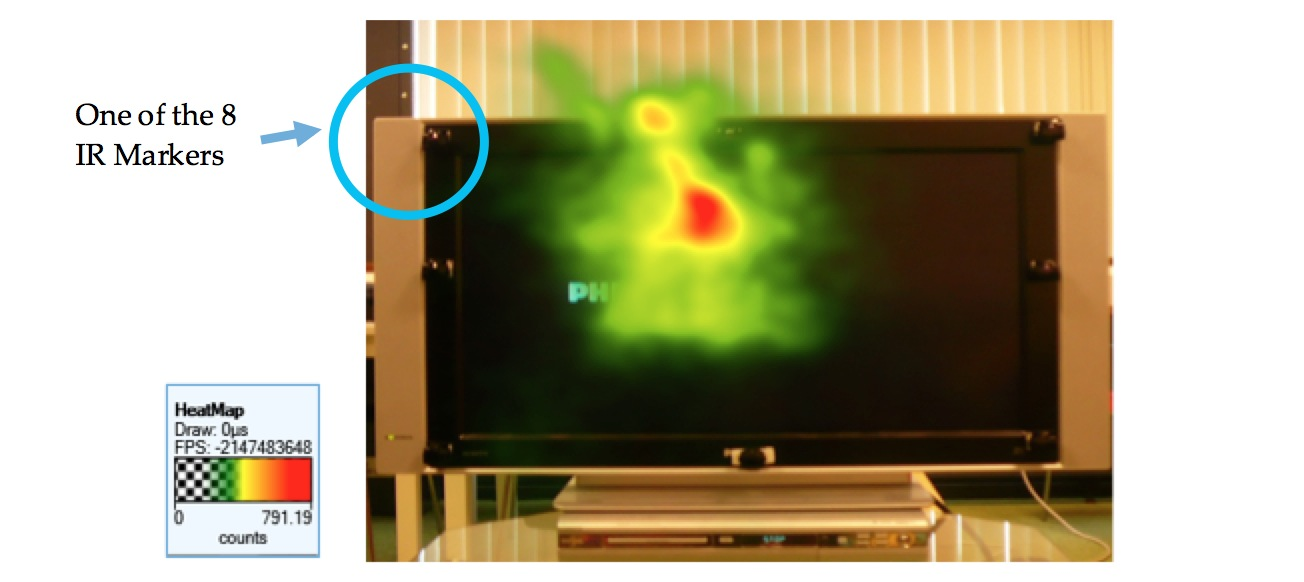
\includegraphics[width=\textwidth]{figures/OHagan2.png}
 \caption{Heatmap of the aggregate fixation of all participants}
 \label{fig:2}
\end{figure}

A heatmap visualization like \ref{fig:2} demonstrates the hot-spots where participants fixated, with the warmest colour (red) showing the most fixations, followed by yellow and then green. This initial observation and the aggregate heatmap helped us to determine areas of interest (AOI) in the subsequent eye-tracking data analysis and facilitated us to form the following post hoc hypotheses:

\begin{enumerate}
\item Eyes frequently fixate in the region of faces in the upper middle region of the screen
\item Visits to the bottom region where impact captions are placed are rather infrequent
\end{enumerate}

Based on these initial observations we set up three AOIs as in \ref{fig:3} for our analysis:

\begin{figure}
 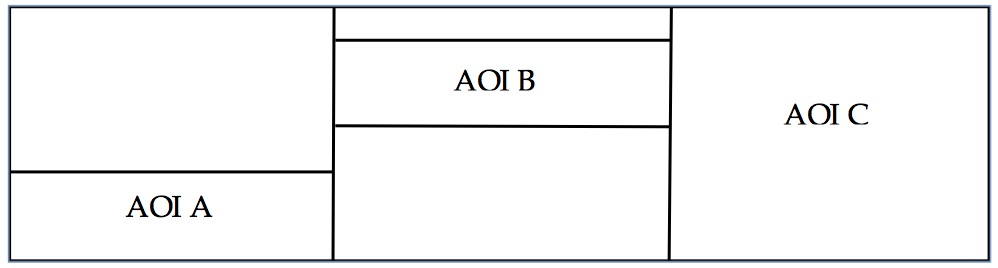
\includegraphics[width=\textwidth]{figures/OHagan3.png}
	\caption{Setting up of three AOIs (AOI A: 1787x434, AOI B 1787x402, AOI C: 1787x1224)}
	\label{fig:3}
\end{figure}

We applied an approach inspired by the above-mentioned study by Josephson and \citet{Holmes2006} who divided the screen for the purpose of analysis according to discrete regions based on the type of TV screen enhancements. Unlike other types of subtitling, impact captions have varying timing, duration and frequency as well as varying appearances as explained earlier.  Because of this reason, we decided to follow a similar approach to Josephson and \citet{Holmes2006} to focus on the distribution of visual attention as a percentage of fixation counts in each region, i.e. fixation counts of each region divided by those of the whole screen.  Tobii's IVT Fixation Filter was applied in this study with the minimum fixation duration set at 100ms. We considered fixation values themselves have little relevance in relation to prior studies which were not focused on this type of caption. Also we compared eye-path cluster patterns of each participant to seek any specific trends.  

\subsection{Results}

A far greater number of fixations was shown in the middle region of the screen than in the bottom caption region in terms of mean number of fixations with M=886 and M=325 respectively for the total valid results from 14 participants. However, in relation to the mean fixation duration the results showed with the middle region slightly shorter than the caption region at M=298ms and M=344ms respectively. For reference purposes the value of mean fixation for "normal reading" is reported as 200-250ms (D'Ydewalle and de Bruycker 2007). Using the ratio of fixation counts of each AOIs (e.g. Caption AOI A and Face AOI B) in relation to the total fixation counts in the whole screen (AOI C) was calculated as shown in \ref{fig:4}. 

\begin{figure}
 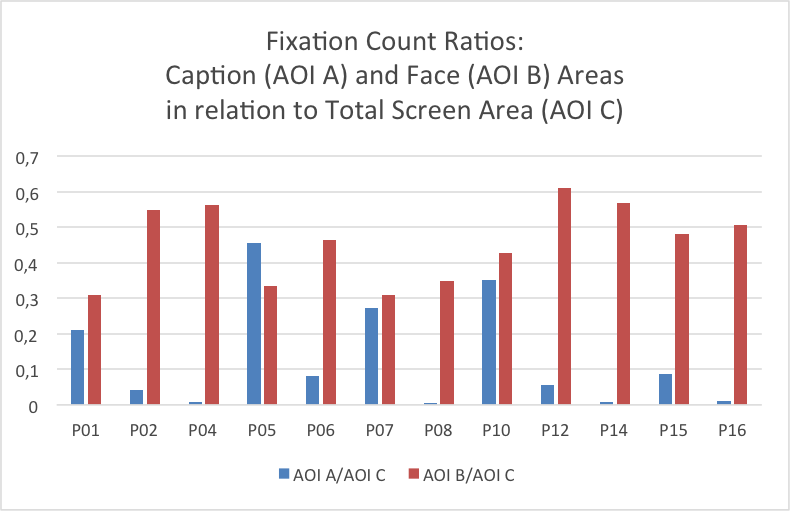
\includegraphics[width=\textwidth]{figures/OHagan4.png}
\caption{Fixation Count Ratio for Caption (AOI A) and Face (AOI B) Areas in relation to Total Screen Area (AOI C) }
\label{fig:4}
\end{figure}

We also calculated the fixation time of the caption area (AOI A) in relation to that of the whole screen area (AOI C) with the mean ratio of all participants (N=14) at 12\%.  However, as illustrated in \ref{fig:5}, the results show a considerable variation according to each participant between 1\% (P4, P8, P14) and 42\% (P5) (SD=14\%).  For information, this compares with 20\% in \citet{D'YdewalleEtAl1991} as previously mentioned. Given the pilot nature of this study these figures may not be fully trustworthy and we did not conduct any statistical analysis. Nevertheless the results gave us a useful indication for our future study and these findings matched our initial observation of the gaze plots and fixation heatmaps, showing that considerably less visual attention was evident in the caption area (AOI A) in comparison to the face area (AOI B) in relation to the fixation on the whole screen.  

\begin{figure}
 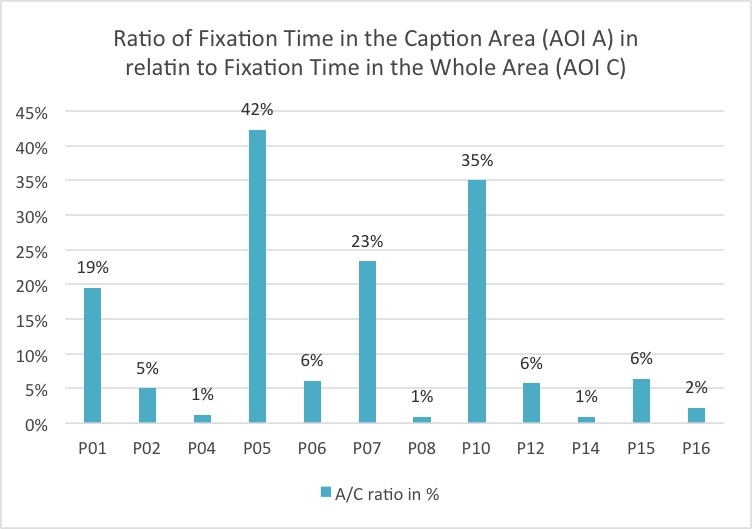
\includegraphics[width=\textwidth]{figures/OHagan5.png}
\caption{Ratio of Fixation Time in the Caption Area in relation to Fixation Time to the Whole Screen}
\label{fig:5}
\end{figure}


The above results therefore seem to confirm our post hoc hypotheses with a far greater number of fixations (2.7 times) in the middle region of the screen where mostly faces are shown.\footnote{ This result might indicate that there are two types of viewers in terms of fixation ratio. However, we could not find any plausible explanation for either group of viewers, in terms of both subjective (self-reported questionnaire) data and objective (eye-tracking) data.} While it does not help explain the viewer impact of the captions, this is in line with the known fact that faces are an eye catcher in that "[f]ace is a natural attention-grabbing visual cue" (Perego et al. 2010, 264). There are also other potential factors such as the nature of the Japanese writing system based on ideographs which may facilitate effective scanning of the key information without fixating on the caption, especially given the large font size typically used (see \ref{fig:1}). However, this is merely speculation and any further investigation was beyond the scope of this paper. In search for possible clues for some marked individual differences we next turned to particular participants.  This led us to pick out the data for P5 showing the greatest fixation in the caption area and compared with P4 who showed the least fixation time in the caption area.  \ref{fig:6} shows the respective heatmap (visualisation based on fixation count) for these two participants where it is evident that P4 tends to fixate on the upper part of the screen whereas P5 in the lower region.

\begin{figure}
 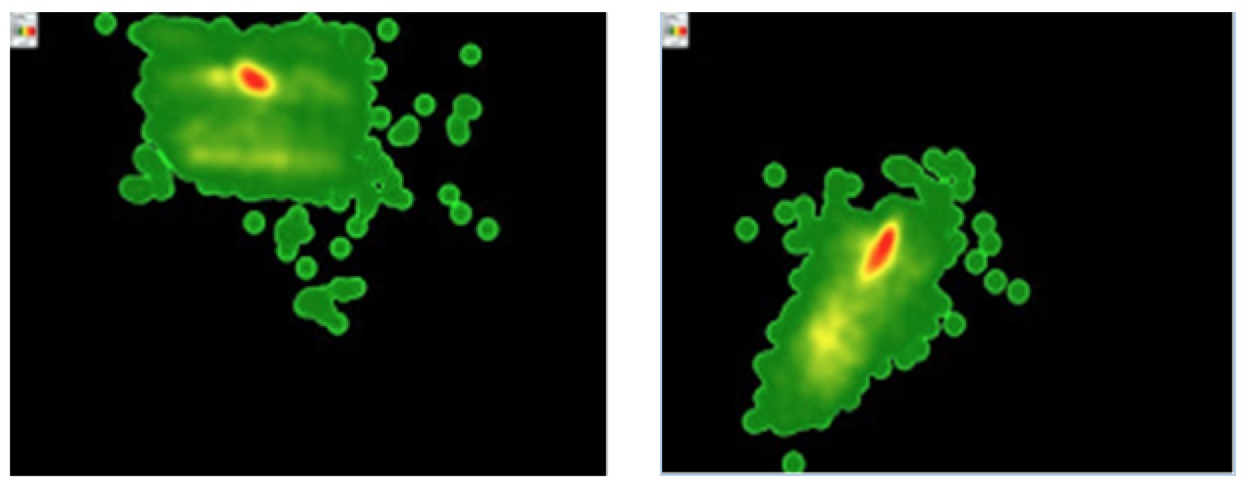
\includegraphics[width=\textwidth]{figures/OHagan6.png}
\caption{Heatmap for P4 (left) versus P5 (right)}
\label{fig:6}
\end{figure}

Figure \ref{fig:7} showing cluster maps for these participants' gaze points is useful in indicating the somewhat different visual attention patterns, further confirming the upper concentration for P4 versus lower for P5.


  
\begin{figure}
 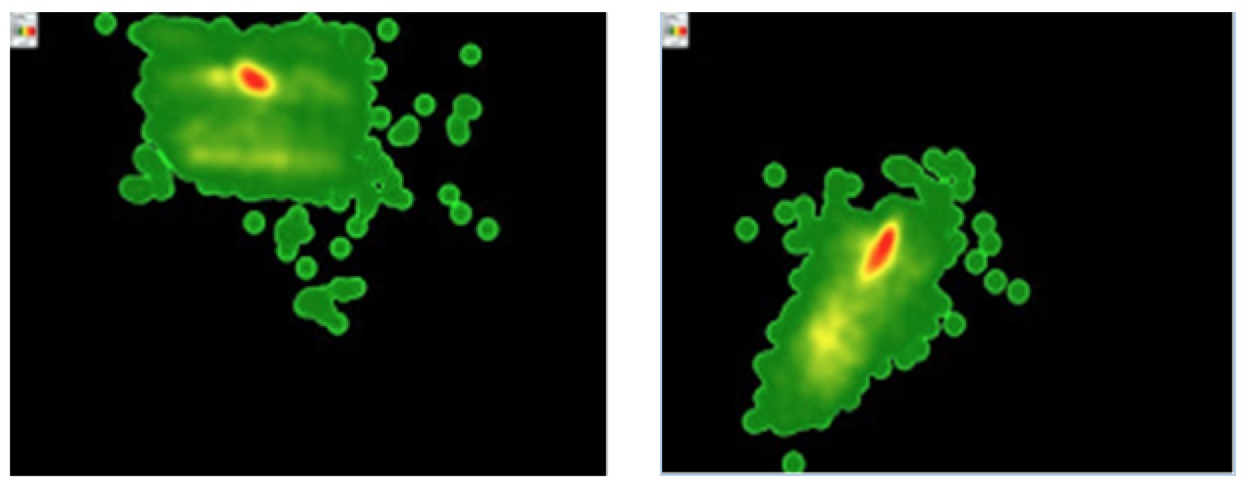
\includegraphics[width=\textwidth]{figures/OHagan6.png}
 \caption{Cluster Maps of Gaze-Paths for P4 (left) and P5 (right)}
\label{fig:7}
\end{figure}


When we cross-checked these participants' questionnaire answers for any marked differences, three questions came to our attention even though they do not directly explain the differences between them in their eye movements; P4 prefers TV programmes that do not use impact captions whereas P5 stated the opposite. However, this preference alone does not seem to justify the markedly high fixations by P5 as most other participants apart from P2 and P4 also admitted they prefer captioned programmes. Regarding whether or not they would normally read impact captions if they are provided, P4 responded that she would read "all" whereas for P5 only those captions which are comments of speakers' utterance. These responses looked somewhat contradictory in relation to their preference for the use of captions in TV programmes: P4 preferred no captions but reads them all if they are there with the eye-tracking data showing few fixations on the captions. However, we did not probe the reasons for their answers. As part of the recall test which asked for the most memorable content P4 was the only respondent who gave the specific name of the chemical in tomatoes (i.e. lycopene) mentioned in the programme. When we checked the gaze plot over the relevant stretch of the programme when lycopene was discussed the gaze plot for P4 did not go to the caption area. Another difference between P4 and P5 was that while P5 would frequently engage in other activities while watching TV, P4 would rarely be engaged in other activities. Both participants chose to say "neither yes nor no" to the question on whether the captions influence their interpretation of the TV content. Incidentally, P4 was female and P5 male. In case of any gender bias we checked the only other male participant (P16) and found no specific shared characteristics between them. Although these answers suggest somewhat different TV viewing habits and preferences, there was no plausible link we could make in relation to the different gaze patterns captured in the eye-tracker.  In summary, the eye-tracking data overwhelmingly showed that eyes very infrequently went to the caption area at the bottom of the screen. 


\section{Discussion}

The eye-tracking experiment was conducted in an explorative study to consider methodological issues as well as to obtain some pointers in understanding the viewers' "reaction" and "response" to the impact captions. Relating to the reception questions, we were particularly interested in shedding light onto (i) viewers' visual attention to impact captions; (ii) factors which potentially affect such attention; and (iii) any notable observable gaze pattern. The fact that there have been no directly relevant prior eye-tracker based studies on these types of TV captions in entertainment rather than news programmes made our study more explorative. 


With potential shortcomings in mind, our results still indicate that viewers generally do not fixate on impact captions nevertheless the participants stated that they would typically read these captions.  Hence, caption reading seems to take place largely outside the foveal vision with aural information likely playing the main role although it is not possible for the eye-tracking data alone to prove this. According to the eye-tracking data the participants were found to fixate far more on the middle screen region where faces were often shown. This could be explained as a natural behaviour of focusing on the image of the speaker than the captions. Although the fixation count is very low in the caption region for most participants, the mean fixation duration is somewhat longer for the captions than for the middle region of the screen with faces, possibly suggesting a somewhat greater cognitive effort for reading the captions. Based on the recall question in the post-task questionnaire most participants were able to recall key topics covered in the programme as well as the number of people who appeared on the programme. This show is particularly designed to deliver new and potentially useful information to the viewers with humour as mentioned earlier, which could prompt affective (emotional) responses from the viewers as also argued on a theoretical basis of cognitive and affective mutuality (Shiota 2003; Sasamoto 2014). In relation to the prior claim that the processing of subtitled films is cognitively effective \citep{PeregoEtAl2010}, our results are inconclusive because of the relatively small amount of fixations in the main caption area even though the viewers were able to demonstrate their comprehension of the content based on some of our recall questions.  Given the highly conspicuous presence of impact captions which were still mostly not fixated we could suggest that the viewers are able to divide their visual attention strategically and not necessarily be drawn to these captions while still taking them in possibly to solidify the aurally gained information.  However, we will clearly need more concrete evidence to soundly prove these points. 



According to the questionnaire responses all the participants had stated that they never mute the sound and simply rely on the captions while all except for one stated that they read all captions or the captions which are offset relating to the speaker's utterance (which consisted of most of our captions used as our stimuli in this study). This implies that these captions are possibly never used as a primary channel for the information, yet the viewers declare they read them. This would therefore be a completely different situation from SDH although there is anecdotal evidence that the elderly population uses these captions to compensate for their reduced hearing (it was assumed that the participants in this study all had good hearing as the demographics of the particular sample were at a relatively young age and confirmed to have normal hearing). An experiment focused on elderly viewers will therefore likely produce different results. We are aware that the way in which our study was designed was not fully conductive to identifying the effect of information redundancy by the use of captions since we did not introduce a control group, which we will need to consider in our future studies.    



Upon reflecting on our method, we wondered if the choice of the particular type of eye-tracker was appropriate although it provided a relatively authentic set-up as all participants admitted that they usually watch TV on TV screens rather than on other devices such as computer screens. Although we were concerned about realism and created a living-room like setup rather than a lab situation, a few things could have been controlled.  For example, a hardback chair may have been more suitable to ensure a more stationary head position than a sofa. We realized that some participants had moved their heads during the recording session despite our instructions to stay still, in some cases affecting the validity of the data which we had to remove. This pointed to the question of trade-off between control and realism, a perennial issue for any lab-based experiments, suggesting a need for more considered selection of eye-tracking tools. Furthermore, we also came to wonder about the particular design of the glass type eye-tracker sometimes proving not a good-fit for Asian facial characteristics often with a lower nose bridge than European counterparts. We note that this issue is addressed in Tobii Glasses 2. These are further points of consideration for future studies. The next question was the issue of the low sampling rate of the eye-tracker at 30 Hz. While it served the purpose of this pilot study, in future we would need to take into account the level of accuracy needed to make a certain claim by capturing more precise eye movement data.  Finally, even though we considered 20 minutes to be a coherent stretch of the stimuli, in future shorter segments may be more productive with the use of control group testing by removing the captions, for example, as in the case of a study by \citet{MatsukawaEtAl2009} to be able to highlight more conclusive observations of the effect of the captions in the context of information redundancy.   


\section{Conclusions}

We set out to apply an eye-tracker-based research methodology in order to shed light onto little discussed TV impact captions now widely used in parts of Asia while attempting to contribute to the lack of empirically-based reception studies in AVT. Although we were unable to arrive at a conclusive finding as to the viewer impact of the impact captions, this pilot study has given us a possible future direction to conduct control experiments whereby doctoring the captions themselves in terms of their presence versus absence. Those who are unfamiliar with these captions will likely find them invasive and even distracting because of their conspicuous nature and yet the participants in the study, who were accustomed to such captions, do not fixate on them although allegedly read them (according to their self-reporting). In this study the participants' eyes were shown to be attracted to the middle region of the screen where faces of people are typically shown despite the obtrusive nature of these impact captions. This further reminds us of the more recent approaches such as with the integrated titles used in the BBC Sherlock series where caption-like texts appear more in the middle region (see Sasamoto 2014; Dwyer 2015).  However, among Japanese TV producers there seems to be tacit understanding that impact captions should not be placed too near the faces of speakers for respect especially in the case of celebrities (Private Communication, Mori 2014).  Such a factor seems to be motivated by socio-cultural reasons rather than from research based on reception studies on the recipients and could form part of an interesting topic of investigation in future. 


When competing information is presented in a way which is taxing on one's cognitive load as shown in the study by \citet{Caffrey2009}, there may be a trade-off in visual attention.  Other studies (Perego et al. 2010, 265) suggest that it may depend on the complexity of the information and the degree of redundancy and "the individuals will not usually encounter serious difficulties in multiple-source information coming from various sources" Our study suggests the latter to be the case in distributing visual attention and dealing with multiple information sources although our stimulus mainly consisted of light entertainment which was unlikely to be taxing on one's cognitive load.  However, the captions themselves presented a complex semiotic unit, combining different colours, style of font and in varying lengths sometimes accompanied by further effects. In a future study these elements will be a worthy focus in shedding further light on the impact of such additional effects on the viewers. 



TV stations in Japan compete to develop a new mechanism to increase viewer ratings on their programmes and the use of impact captions is part of such a strategy to differentiate their programmes from the competition's (Private Communication, Mori 2014). Although we acknowledge the limitation of this study relating to the capacity of the eye-tracker and our method, it showed a potential for these tools to be used to inform TV producers how their captioned programmes are received physiologically by viewers and in turn potentially informing their future caption strategies.  



In translation studies there is an increasing interest in user response to translation, for example, as proposed as "user-centred translation" (Suojanen, Koskinen and Tuominen 2015) in which user experience (UX) informs translation strategies. While UX has been an area of interest in the field of human computer interaction (HCI) it is currently under explored in translation studies, suggesting a fruitful avenue for research (O'Hagan and Mangiron 2013, 312-318). This pilot study gave us an opportunity to further such an anchor on users and to provide clues for methodological consideration for such future studies using eye-tracking in AVT contexts. 


Acknowledgement

This study was funded by the Research Support Office at Dublin City University under the 2013 Career Enhancement Award, and by the Faculty of Humanities and Social Sciences under the Performance Enhancement Scheme 2013. We would also like to acknowledge Dr. Stephen Doherty, from the University of New South Wales, for his contribution to this research project, and DCU doctoral researcher Mr. Feiyan Hu for his technical assistance with the eye-tracking tool. However, any errors and omissions are our own. 

\section{References}


Bisson, Marie-Josee; Van Heuven, Walter J. B.; Conklin, Kathy and Richard J. Tunney. 2014. Processing of native and foreign language subtitles in films: An eye tracking study. \textit{Applied Psycholinguistics} 35, 399-418.



Caffrey, Colm. 2009. \textit{Relevant abuse? Investigating the effects of an abusive subtitling procedure on the perception of TV anime using eye tracker and questionnaire}. A PhD thesis submitted at Dublin City University. 



D\'{i}az-Cintas, Jorge. 2013. Subtitling: Theory, practice and research.  In \textit{The Routledge Handbook of Translation Studies}, ed. by Mill\'{a}n, Carmen and Francesca Bartrina, 273-287. London and New York: Routledge.



Dwyer, Tessa. 2015. From Subtitles to SMS: Eye Tracking, texting and Sherlock. \textit{Refractory: A journal of entertainment media} vol. 25, n.p. http://refractory.unimelb.edu.au/2015/02/07/dwyer/ 



D'Ydewalle, G., \& Gielen, I. 1992. Attention allocation with overlapping sound,image, and text. In \textit{Eye movements and visual cognition: Scene perception and reading}, ed. by Rayner, Keith, 415-427. New York: Springer-Verlag.



D'Ydewalle, G., \& De Bruycker, W. 2007. Eye movements of children and adults while readingtelevision subtitles. \textit{European Psychologist}, 12, 196-205.



Fox, Wendy. 2013. Integrated Titles as an Alternative Solution to Traditional Subtitles. Paper presented at \textit{the 7}\textit{\textsuperscript{th}}\textit{ EST Conference - Translation Studies: Centers and Peripheries}, Germersheim, Germany.



Gambier, Yves. 2008. Recent developments and challenges in audiovisual translation research. In \textit{Between Text and Image: Updating research in screen translation}, ed. by Chiaro, Delia, Heiss, Christine and Chiara Bucaria, 11-33. Amsterdam and Philadelphia: John Benjamins. 



Gambier, Yves. 2013. The position of audiovisual translation studies. In \textit{The Routledge Handbook of Translation Studies}, ed. by Mill\'{a}n, Carmen and Francesca Bartrina, 45-59. London and New York: Routledge.



Ghia, Elisa. 2012. The Impact of Translation Strategies on Subtitle Reading. In \textit{Eye Tracking in Audiovisual Translation}, ed. by Elisa Perego, 155-182. Roma: Aracne Editrice. 



Jakobsen, Arnt Lykke. 2014. The development and current state of translation process research. In \textit{The Known Unknowns of Translation Studies}, ed. by Brems, Elke, Meylaerts, Reine and Luc van Doorslaer, 65-88. Amsterdam \& Philadelphia: John Benjamins.



Jensema, Carl. J., Sharkawy, El Sameh., Sarma Danturthi, Ramalinga, Burch, Robert. and Hsu, David. 2000a. Eye movement patterns of captioned television viewers. \textit{American Annals of the Deaf}. 145 (3), pp 275-285.



Jensema, Carl.J., Sarma Danturthi, Ramalinga., and Burch, Robert. 2000b. Time spent viewing captions on television programs. \textit{American Annals of the Deaf}. 145 (5), pp 464-468.



Josephson, Sheree and Holmes, Michael, E. 2006. Clutter or content? How on-screen enhancements affect how TV viewers scan and what they learn. In \textit{ETRA '06 Proceedings of the 2006 symposium on Eye Tracking Research \& Applications (ETRA)}, 155-162. San Diego, California, 27-29 March 2006.



Kato, Masao. 2012. \textit{??? [Japanese Language on TV]}. Tokyo: Iwanami Shinsho.



Kimura,Tamako, Hosoi, Akiko., Honda, Naoko., Kato, Yuri., Kawamura, Fumiko., Koizumi, Aya., Oosawa, Yukoko., Suzuki, Eri. and Kaori Watabe. 2000. ?????????????????????????????????[305F?]??????[751F?]????????? [Physiology of Letters Dancing on TV screen], \textit{Galac} 35.



Kova\v{c}i\v{c} Irina. 1995. Reception of Subtitles: The non-existent ideal viewer. \textit{Translatio} 14 (3-4), 376-383.



Kruger, Jan Louis, Aszarkowska, Gnieszka and Krejtz, Izabela. 2015. Subtitles on The Moving Image: An overview of eye tracking studies\MakeUppercase{.}\textit{Reflactory: A journal of entertainment media} vol. 25, n.p. \url{http://refractory.unimelb.edu.au/2015/02/07/kruger-szarkowska-krejtz/}



Kruger, Jan-Louis and Faans Steyn. 2014. Subtitles and Eye Tracking: Reading and Performance. \textit{Reading Research Quarterly} 49 (1): 105-120.



K\"{u}nzli, Alexander and Ehrensberger-Dow, Maureen. 2011. Innovative subtitling. A reception study. In \textit{Methods and Strategies of Process Research}, ed. by Alvstad, Cecilia, Hild, Adelina and Elisabet Tiselius. Amsterdam: John Benjamins. 187 - 200.



Maree, Claire. 2014. ????????????[305F?]????????? [I want to transform myself]???. \textit{???????????????[4F1A?] [Languages and Society]} 16: 57-85.



Maree, Claire. 2015. "The Perils of Paisley and Weird Manwomen: Queer Crossings into Primetime J-TV via Telops" In \textit{Multiple Translation Communities in Contemporary Japan}, eds. by Curran, Beverley, Sato-Rossberg and Kikuko Tanabe, pp. 124-147. New York and London: Routledge.



Matsukawa, Rei, Miyata, Yosuke and Ueda, Shuichi. 2009. Information Redundancy Effects on Watching TV News: Analysis of Eye Tracking Data and Examination of Contents. \textit{Library and Information Science}, 62, 193-205. 



Mayer, Richard. E. and Moreno, Roxana. 1998. A split attention effect in multimedia learning: evidence fo dual processing systems in working memory. \textit{Journal of Educational Psychology}, 902, 312-320.



Nielsen, Jakob and Pernice, Kara. 2010. \textit{Eyetracking Web Usability}. Berkeley, CA: New Riders.



O'Hagan, Minako. 2010. "Japanese TV Entertainment: Framing Humour with Open Caption Telop" In \textit{Translation, Humour and the Media}, ed. by Chiaro, Delia, pp. 70-88. London: Continuum.



O'Hagan, Minako and Mangiron, Carmen. 2013. \textit{Game Localization: Translating for the global digital entertainment industry}. Amsterdam and Phladelphia: John Benbajims.  



Orrego-Carmona, David. 2014. Where is the audience? Testing the audience reception of non-professional subtitling. In \textit{From Translation Research Projects 5}, ed. by Torres-Simon, Esther and David Orrego-Carmona, 77-92. Tarragona: Intercultural Studies Group.



Park, J S-Y. 2009. "Regimenting Lanuages on Korean Televison: Subtitles and Institutional Authority" Text \& Talk 29 (5): 547-570. 



Pedersen, Jan. 2011. \textit{Subtitling Norms for Television: An exploration focussing on extralinguistic cultural references}. Amsterdam \& Philadelphia: John Benjamins



Perego, Elisa, Del Missier, Fabio, Porta, Marco and Mosconi, Mauro. 2010. Cognitive Effectiveness of Subtitle Processing. \textit{Media Psychology} 13: 243-272



Perego, Elisa. 2012 (ed.). \textit{Eye-tacking in Audiovisual Translation}. Roma: Aracne Editrice.



P\'{e}rez-Gonz\'{a}lez, L. 2012. "Co-creational subtitling in the digital media: transformative and authorial practices" International Journal of Cultural Studies. 16 (1), 3-21.



Sakamoto, Mamoru.1999. ???[6FEB?]?????????????????????[529F?][7F6A?] [Benefit and Sin of Overuse of Subtitled Programmes]. \textit{Galac} 359, 36-39.



Sasamoto, Ryoko. 2014. Impact caption as a highlighting device: Attempts at Viewer Manipulation on TV. \textit{Discourse, Context and Media} 6: 1-10.



Shiota, Eiko. 2003.?????????????????????????????????????????? [Relevance theory and understanding of telop] Journal of Ryukoku University, 63-91.



Shitara, Kaoru. 2012. Changes in the use of Telop observed with NHK Variety Programmes. \textit{Mukogawa Joshidai Journal} 59.



Sperber, Dan and Deirdre Wilson. 1986/1995. Relevance: Communication and Cognition. Oxford: Blackwells.



Suojanen, Tytti, Koskinen, Kaisa and Tiina Tuominen. 2015. \textit{User-centred Translation}. London: Routeldge.



Tobii Glasses Eye Tracker User Manual. 2012. Tobii Technology AB.  \url{http://www.tobii.com/Global/Analysis/Downloads/User_Manuals_and_Guides/Tobii Glasses User Manual.pdf}



Treisman, Anne, M. 1968. Strategies and models of visual attention. \textit{Psychological Review}, 84, 127-190.


\subsection*{Abbreviations}
\subsection*{Acknowledgements}

\printbibliography[heading=subbibliography,notkeyword=this]

\end{document}